\begin{figure}[htbp]
  \centering
  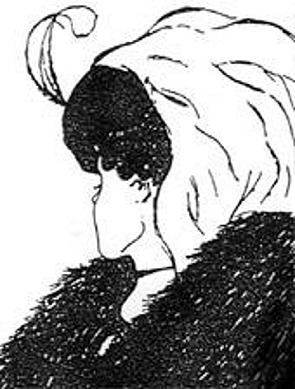
\includegraphics[width=0.48\textwidth]{src/images/youngoldwoman.jpg}
  \caption[妻と義母（若い女性と老婦人）]{「妻と義母」（若い女性と老婦人）：輪郭線や陰影の局所的特徴量 $D$ に対し、事前仮説 $H_{\text{young}}$（背後を向く若い女性）と $H_{\text{old}}$（横顔の老婦人）が同一の入力に対して競合する多峰性認知の代表例。\newline
  {\footnotesize 出典: W.~E.~Hill, \textit{Puck}（1915年11月6日号）, Public Domain.}}
  \label{fig:wife_and_mother_in_law}
\end{figure}
